%
% ggt.tex -- GGT, Definition und Algorithmus
%
% (c) 2021 Prof Dr Andreas Müller, OST Ostschweizer Fachhochschuöe
%
\begin{frame}[t]
\frametitle{Grösster gemeinsamer Teiler}
\vspace{-15pt}
\setlength{\abovedisplayskip}{5pt}
\setlength{\belowdisplayskip}{5pt}
\begin{columns}[t,onlytextwidth]
\begin{column}{0.48\textwidth}
\begin{block}{Definition}
Gegeben: $a,b\in\mathbb Z$
\\
Gesucht: grösster gemeinsamer Teiler $\operatorname{ggT}(a,b)$
\end{block}
\uncover<4->{%
\begin{block}{Euklidischer Algorithmus}
$a_0 = a$, $b_0=b$
\begin{align*}
\uncover<5->{
a_0&=b_0q_0 + r_0 & a_1 &=b_0 & b_1&=r_0}\\
\uncover<6->{
a_1&=b_1q_1 + r_1 & a_2 &=b_1 & b_2&=r_1}\\
\uncover<7->{
a_2&=b_2q_2 + r_2 & a_3 &=b_2 & b_3&=r_2}\\
\uncover<8->{
   &\;\vdots      &     &     &    &    }\\
\uncover<9->{
a_n&=b_nq_n + r_n & r_n &= 0  & r_{n-1}&=\operatorname{ggT}(a,b)}
\end{align*}
\end{block}}
\end{column}
\begin{column}{0.48\textwidth}
\begin{block}{$\operatorname{ggT}(15,25) = 5$}
\begin{center}
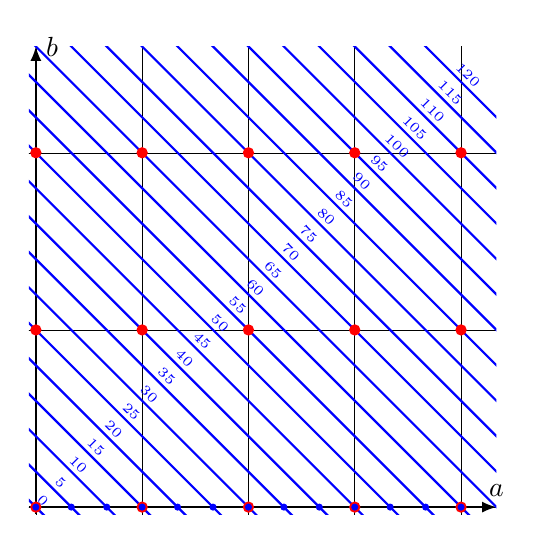
\begin{tikzpicture}[>=latex,thick,scale=0.09]
\draw[->] (-1,0) -- (65,0) coordinate[label={$a$}];
\draw[->] (0,-1) -- (0,65) coordinate[label={right:$b$}];
\begin{scope}
\clip (-1,-1) rectangle (65,65);
\foreach \x in {0,...,4}{
	\draw[line width=0.2pt] ({\x*15},-2) -- ({\x*15},65);
}
\foreach \y in {0,...,2}{
	\draw[line width=0.2pt] (-2,{\y*25}) -- (65,{\y*25});
}
\uncover<3->{
	\foreach \x in {0,5,...,120}{
		\draw[color=blue] ({\x+2},-2) -- ({\x+2-70},{-2+70});
		\node[color=blue] at ({0.5*\x-0.5},{0.5*\x-0.5})
			[rotate=-45,above] {\tiny $\x$};
	}
}
\uncover<2->{
	\foreach \x in {0,...,4}{
		\foreach \y in {0,...,2}{
			\fill[color=red] ({\x*15},{\y*25}) circle[radius=0.8];
		}
	}
}
\uncover<3->{
	\foreach \x in {0,5,...,60}{
		\fill[color=blue] (\x,0) circle[radius=0.5];
		\node at (\x,0) [below] {\tiny $\x$};
	}
}
\end{scope}
\end{tikzpicture}
\end{center}
\end{block}
\end{column}
\end{columns}
\end{frame}
